\begin{figure}[H]
	\centering
	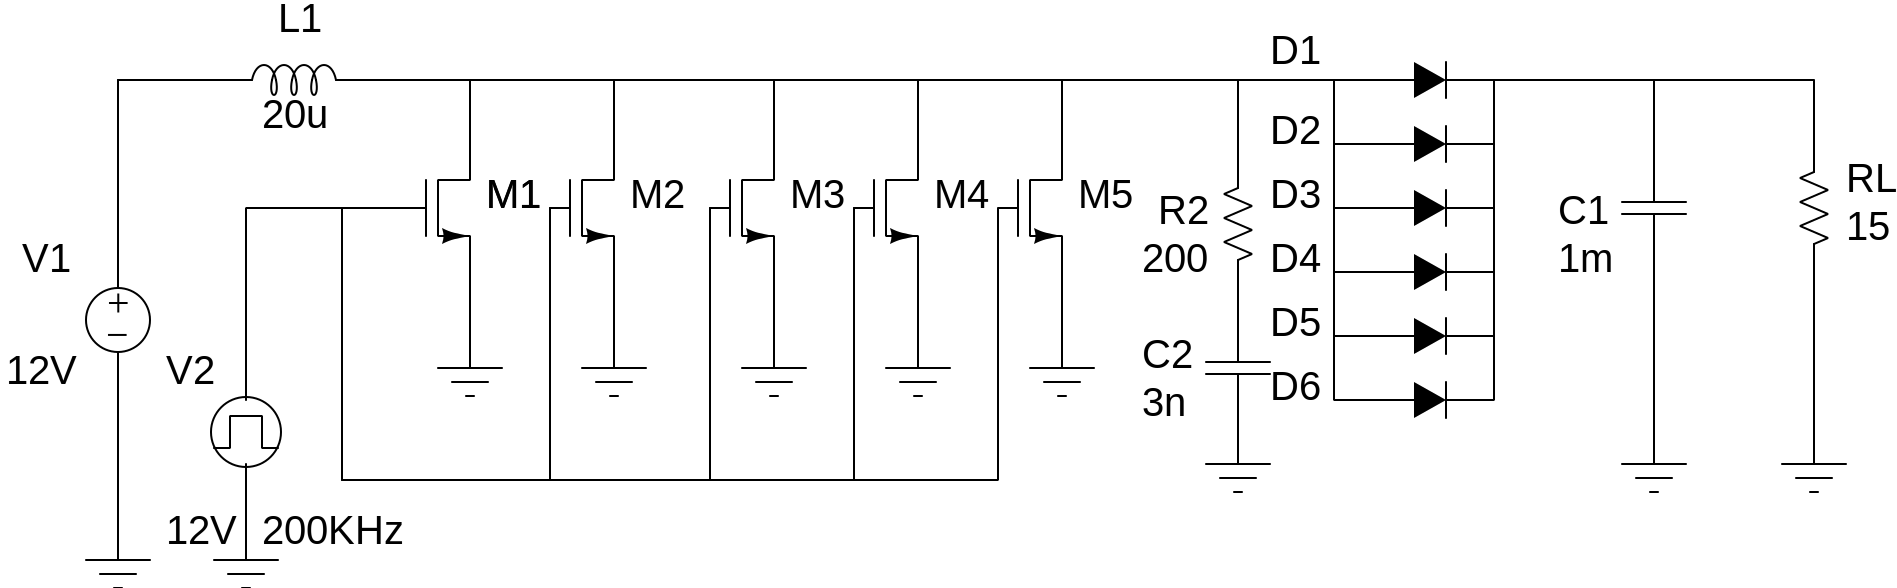
\includegraphics[scale=0.3]{Circ2}
	\caption{Circuito completo.}.
	\label{fig:Circ2}
\end{figure}


El circuito del Esquema \ref{fig:Circ2} corresponde a un regulador \textit{Flyback}. Su funcionamiento puede analizarse en dos ciclos. 

\begin{itemize}
	\item \textbf{Primer ciclo:} cuando la señal de pulso toma el valor de \SI{12}{\volt}, $V_{GS}=\SI{12}{\volt}$ por lo que el MOSFET está en conducción. El diodo $D$ se encuentra polarizado en inversa y la corriente que circula por el inductor produce almacenamiento de energía en su núcleo. El circuito simplificado se representa en la Figura \ref{fig:1ciclo}.

		Es posible calcular la corriente en el inductor máxima, sabiendo que el pulso tiene una frecuencia de \SI{20}{\kilo\hertz} y que posee medio ciclo de trabajo.

		\begin{equation}
			\centering
			I_{L1}(t) = \frac{V_1}{R_{DS<on>}} \left(1-\exp{(-t/\tau)}\right),
		\end{equation}
		siendo $t_{carga} = \tau=L1/R_{DS<on>} = \SI{533}{\micro\second}$. El periodo del pulso es $\SI{50}{\micro\second} < t_{carga}$
entonces la corriente máxima en el inductor es

		\begin{equation}
			\centering
					I_{L1}(\SI{25}{\micro\second}) = \frac{\SI{12}{\volt}}{\SI{0.0375}{\ohm} } \left(1-\exp{(\SI{-25}{\micro\second}/ \SI{533}{\micro\second})}\right) = \SI{14.7}{\ampere}
		\end{equation}

	
\HgraficarEPS{0.5}{cto_ej2_1ciclo}{Primer ciclo}{fig:1ciclo}


\item \textbf{Segundo ciclo:}
	Cuando el pulso vale \SI{0}{\volt}, el MOSFET se encuentra en corte, lo cual equivale a una impedancia muy elevada. Debido a que la corriente en el inductor no puede cambiar instantáneamente, se invierte la polaridad de la tensión en el inductor y el diodo pasa a estar en directa. Se produce una transferencia de energía desde el inductor al capacitor hasta que el inductor se descargue por completo. Debido a que la tensión en el inductor se invierte (\textit{flies back}), la tensión en la salida es mayor que la de entrada. El circuito simplificado se muestra en la Fiugra \ref{fig:2ciclo}.

\HgraficarEPS{0.5}{cto_ej2_2ciclo}{Segundo ciclo}{fig:2ciclo}

		El regulador opera en modo discontinuo, por lo que el inductor se descarga completamente en cada ciclo, es decir que la corriente en el inductor se anula. El comportamiento de la corriente en el inductor se ilustra en la Figura \ref{fig:mod_dis}. El tiempo de descarga debe ser menor al de carga. $T > t_{carga} + t_{descarga}$, considerando $t_{descarga} = \SI{10}{\micro\second}$, el valor de $D$ (\textit{duty cycle}) es 

		\begin{equation}
			\centering
			D = \frac{t_{carga}}{t_{carga} + t_{descarga}} \cong \boxed{\num{0,7}}
		\end{equation}
		
	%	\Flor{Encontré esta fórmula, que es parecida a (17)}
	%	La tensión de salida puede aproximarse

	%	\begin{equation}
	%		\centering
	%		V_S \cong V_E \left( 1 + \frac{t_{carga}}{t_{descarga}} \right) = \SI{12}{\volt} \left(1+ \frac{25}{15}\right) = \boxed{\SI{32}{\volt}}
	%	\end{equation}
\end{itemize}


\HgraficarEPS{0.6}{modo_discontinuo}{Modo discontinuo}{fig:mod_dis}


%\Gus{Tiro ecuaciones que seguro se van a usar, al menos son las que use para intentar el calculo}
%\Flor{Creo que estas ecuaciones no se usan}
%
%\begin{equation}
%	{L} = \frac{(1-D) \cdot (V_s - V_E)}{2 \cdot f \cdot (I_{L_{max}} - I_{L_{prom}})}
%\end{equation}
%
%\Gus{verificar esta ecuacion}
%\begin{equation}
%	V_s = \frac{(V_E - V_{sat})}{1-D} - V_D \cdot (1 - D) 
%	\label{ec:Nose}
%\end{equation}
%
%\Flor{En la diapo está un toque distinta}
%
%\textcolor{blue}{$$V_S = (V_E-V_{SAT}) \left(  1 + \frac{t_{carga}}{t_{descarga}} \right) -V_D$$}
%
%\Gus{Grafico XX de $I_S$ respecto al tiempo tengo que sacarlo de las diapos}

La corriente de salida está dada por \eqref{ec:is}.
\begin{equation}
	I_s = \frac{I_{max} \cdot (1-D) \cdot T}{2 \cdot T} = \frac{I_{max} \cdot (1 - D)}{2} 
	\label{ec:is}
\end{equation}

Al estar trabajando en modo discontinuo se cumple que $ 2 I_{L_{prom}} =I_{L_{max}} $ por lo tanto.


\begin{equation}
	L = \frac{(1 - D)^2 \cdot (V_s - V_E)}{2 \cdot f \cdot (I_s)}
\end{equation}

Despejando y tomando a $\frac{V_s}{I_s} = R_L = \SI{15}{\ohm}$


\begin{equation}
	I_s^{-1} = \frac{\SI{15}{\ohm} - \frac{L \cdot 2 \cdot f}{(1-D)^2}}{V_E}
\end{equation}

Con $D=0,7$

\begin{equation}
	\boxed{I_s = \SI{1,963}{\ampere}}
\end{equation}


\begin{equation}
	\boxed{V_s = R_L \cdot I_s = \SI{29,45}{\volt}}
\end{equation}

